\documentclass[]{article}

% math packages
\usepackage{amsmath}
\usepackage{amsthm}
\usepackage{bm}

% including graphics
\usepackage{graphicx}
\graphicspath{ {./images/} }

% drawing graphs
\usepackage{tikz-cd}
\usepackage{tikz}
\usetikzlibrary{shapes.geometric, arrows}
\tikzstyle{startstop} = [rectangle, rounded corners, minimum width=3cm, minimum height=1cm,text centered, draw=black, fill=red!10]
\tikzstyle{arrow} = [thick,->,>=stealth]

% some useful shortcuts
\DeclareMathOperator*{\argmax}{argmax}
\newcommand{\indep}{\perp\!\!\!\!\perp}
\newcommand{\blambda}{{\bm{\lambda}}}
\newcommand{\btheta}{{\bm{\theta}}}
\newcommand{\bpsi}{{\bm{\psi}}}

\newcommand{\by}{\mathbf{y}}

\usepackage{setspace}
\doublespacing

% Editing macros
\usepackage{color}
\newcommand\cmnt[2]{\qquad{{\color{red} \em #1---#2} \qquad}}
\newcommand\cmntM[1]{\cmnt{#1}{Miratrix}}
\newcommand\cmntC[1]{\cmnt{#1}{Che}}
\newcommand\awk{{{\color{red} {$\leftarrow$ Awkward phrasing}}\qquad}}
\newcommand\cmntMp[1]{{\color{red} $\leftarrow$ {\em #1 -Miratrix} \qquad}}



%opening
\title{Power calculations for detecting \\ individual site impacts}
\author{Jonathan Che \& Luke Miratrix}

\begin{document}
	
\maketitle

%\begin{abstract}
%\end{abstract}


\section{Introduction}

The usual question for a multisite trial, those randomized trials where each of a set of sites has individuals randomized into treatment and control, is whether the treatment worked \emph{on average overall}.
Even this question has its wrinkles, if we believe the site-level average effects differ.
For example, do we estimate the average impact for all individuals across all sites, or instead estimate the simple site average of their average impacts?
Regardless, when designing a multisite experiment there are power analysis tools designed to ensure a given design will achieve desired levels of power for these average effects.
There are even power formulas designed to ensure one can detect a given level of cross-site impact variation, if that is a quantity of interest.

But what if we are interested in the individual sites?
Typically, in a multisite experiment no individual site will be large enough to be well-powered, on its own, for detecting whether that site was actually effective.
This is, after all, why we frequently turn to multisite experiments: we seek to increase our overall power by averaging across a suite of underpowered, local, investigations.
That being said, the stakeholders at these local investigations will frequently want to know not whether the experiment worked overall, but whether it worked for them.
As researchers, we might also want to identify which sites are most likely to be the drivers of an overall effect.

An approach to answering, at least approximately, these individual-site focused questions is to use multilevel modeling, or hierarchical Bayesian modeling, to partially pool the individual site effects.
We hope to ``borrow strength'' from the other sites, making the assumption that the sites are related and thus their true impacts are likely more similar than what we see given the overall uncertainty.
This process results in point estimates, with nominal uncertainty measures, for each of the individual sites that are shrunken towards the overall average estimated effect.
These shrunken estimates and corresponding intervals will be biased, meaning they will not necessarily have good control over error rates.
But they might be better than nothing.

While there is an extensive literature on power analyses for the overall average treatment effect and cross-site variation in multisite trials (e.g., Raudenbush \& Liu 2000, many others...), less attention has been paid to inferences for these individual estimates.
Particularly, how to calculate the power to detect a hypothesized effect for a specific site in a particular study design is not entirely clear.
In this paper we explore using multilevel and Bayesian modeling to report on individual site impacts.
We first review how one might model and report such effects.
We then propose simulation-based tools to do power calculations.
We then conduct a simulation study to examine individual level power for site-level treatment effects in multisite trials.
At this point, we also examine how poorly these individual level estimates perform in practice, and provide guidance on the overall business of individual site estimation in the context of multisite trials.


\section{Detecting individual site effects}

Assume a model for individuals $i$ in sites $j$, where we fix  $Var(Y(0)) = 1$ (to be in effect size units), of 
\begin{align*}
	Y_{ij} &= \alpha_j + \tau_j Z_{ij} + \epsilon_{ij} \\
	\alpha_j &= \alpha + u_{0j} \\
	\tau_j &= \tau + u_{1j} \\
	\begin{pmatrix}
		u_{0j} \\ u_{1j}
	\end{pmatrix} &\sim N\left(
	\begin{pmatrix}
		0 \\ 0
	\end{pmatrix}, 
	\begin{bmatrix}
		ICC & \rho \\ \rho & \omega
	\end{bmatrix}\right) \\
	\epsilon_{ij} &\sim N(0, 1-ICC) ,
\end{align*}
where $Z_{ij}$ are the individual treatment indicators, $\tau$ is the overall site-average treatment impact, and $\omega$ is the amount of cross site variation.
The $u_{0j}$ are the random intercepts for the sites, and the $u_{1j}$ are how the sites vary from each other in terms of average treatment impact.

The effect size scaling gives the variance of our random intercepts in terms of the Intra Class Correlation Coefficient (ICC) of
$$ ICC = \frac{Var(\alpha_i)}{Var(\alpha_i) + Var(\epsilon_{ij})} = Var(\alpha_i) .$$
This also dictates that our within-site residual variation $\sigma^2$ is $1-ICC$.
We ignore additional covariate adjustment for the moment for transparency.

The simplest, completely unpooled test of whether an individual site had a positive effect would be to drop the rest of the data and test the difference in means of the treatment and control groups at that site.
The power to detect effects locally in this manner is purely a function of the site sample size, site variation, and the size of the true average impact.
The standard error for Site $j$'s impact estimate would then be
$$ SE_j = \left[ \frac{1}{n_j} \frac{1}{(1-p_j)p_j} (1-ICC) \right]^{1/2} , $$ 
where $p_j$ is the proportion treated at site $j$.

For testing, we would estimate $\hat{\tau}_j$ and $\widehat{SE}_j$, the latter with a plug-in estimate of $\hat{\sigma}_j$.
We obtain $p$-values using $t = \hat{\tau}_j / \widehat{SE}_j$, referenced to a $t$ distribution with many degrees of freedom, assuming the site is not tiny.
(We could estimate $\hat{\sigma}_j$ (the $1 - ICC$ term) with an interacted linear regression where we completely pool our residual variation across sites, or simply estimate the within-group variation at site $j$. The former would help stabilize, under homoscedasticity, our residual estimate which could be helpful in very small sample contexts.)

A multisite analysis does none of this, of course.
Instead, with a multilevel model, we initially estimate the overall parameters, including $\omega$, the degree of cross site variation, and none of the individual site average impacts.
We then, in a second step, effectively shrink all the raw $\hat{\tau}_j$ towards the overall estimate of $\hat{\tau}$, shrinking more the lower our estimate of $\omega$ is.
These $\tilde{\tau}_j$ are the Empirical Bayes estimates for the individual site impacts; while biased, they are known to be better predictors of the full collection of true site-level impacts than the raw estimates, above.

We can also obtain (poorly performing) standard error estimates $\tilde{SE}_j$ for our $\tilde{\tau}_j$ as well.
Using the estimate and standard error, we can finally conduct hypothesis testing as before, taking the test statistic of $t = \tilde{\tau}_j / \tilde{SE}_j$ as standard normal statistic and calculating a $p$-value as usual.
These tests will not, however, have the usual guarantees on error rate control.
That being said, they may perform decently well in practice.

Without shrinkage, power is simply a function of the un-shrunk standard error $SE_j$ and the true average effect $\tau_j$ for site $j$.
Given the shrinkage, the power to detect an individual site effect will additionally depend on the  the general size and distribution of average effects at other sites.
Of course, the most relevant parameter will be the site's average effect, but the distribution of impacts estimated at the other sites will affect how each site estimate is shrunk towards the overall average impact.
The question is how much this shrinkage helps or hurts the power and validity of the testing procedure, especially for those sites that actually have impacts far from the overall average.


\section{A simulation-based power calculator}

To assess power for a hypothesized individual site, we need to specify the site we are estimating power for, as power for a site depends primarily on the true impact for the site.
In the multilevel modeling case, we also need to specify the \emph{context} that the site is in, as the overall context will also affect our individual estimate and uncertainty estimate.
I.e., overall we will need to specify the characteristics, including the individual true site impact, for a target site, and then also specify the number of additional sites, the distribution of site effects, and so forth, that our target site resides in.
We can then ask, for the given site of interest, for the context of interest, what is the chance of rejecting the null of no effect for that site?
We do this via simulation: we repeatedly generate our target site and the associated context, analyze the synthetic data, and record whether we have detected an effect.
The frequency we reject the null across our simulations is the power for that site and context.
We propose two general tools for conducting such a simulation.


\paragraph{Set site simulation.} A straightforward way of doing this is to specify the site, and then separately specify the distribution of sites in the context.
This decouples the site from context: we could in principle ask the chance of noticing a large impact in a context where all the rest of the sites have no impact.
This does mean the overall true treatment effect for our simulated samples will be a weighted average between our fixed site effect and the mix of additional sites generated.
That being said, the set site approach allows for a straightforward specification of these two components.

\paragraph{All site simulation.} For power calculations, we often want an entire power curve, where we can see the power to detect a range of possible impact sizes.
We can generate such a curve in a single step by repeatedly generating full multisite datasets, testing all the sites, and then grouping sites with the same true average impact across all the simulation runs.
I.e., if we identify all sites with a given true effect across all runs, we can estimate power for that effect size by calculating the rejection rate across the identified set.
Of course, given the continuous nature of random impact estimate, sites will never have the exact same value.
We therefore round the randomly generated $\tau_j$ to the nearest 0.05 before generating the individual responses within sites.

This approach has a few small caveats: first, we will only obtain power estimates for impact sizes that are in the range we might naturally see given the overall specification of average impact and cross-site variation.
This seems a reasonable limitation, in general, as we want our individual specification to align with the global one.

There is also a slight ``double-booking'' effect in the joint simulation, especially for impact sizes that are much higher or lower than the overall average.
In these cases,  most sites with impacts of a specified unusual size across our simulation runs will be in contexts where the overall average is also more unusual (far from the target $\tau$) because the individual site is part of the overall average.
This bias will be more pronounced with fewer sites, as the individual site will play a larger role.
This double-booking is explicitly being done in the set site simulation approach.
Here it is happening partially, and organically.
\cmntC{This is a good point -- e.g., for a very low treatment effect, the ATE will be slightly lower than usual, so shrinkage will be slightly less than usual.
Perhaps this means that `set site simulation' is the cleaner way to proceed}



\paragraph{Conducting the simulation.}
To generate multisite data, we use the \texttt{blkvar} package in R; this package provides a host of methods for generating multisite data and analyzing it with a variety of models.
We first generate our collection of sites, then round site impacts to the nearest 0.05, and then generate the individuals within the site.
We finally take the generated data and analyze it with whatever planned analytic approach we have decided on.

\section{Simulation}
To understand how multilevel modeling potentially helps power and also undermines control of error rates, we conducted a multifactor simulation across a range of  scenarios.

%The parameters we vary are:
%\begin{itemize}
%	\item $\bar{n}$: the average number of students per site
%	\item $J$: the total number of sites
%	\item $ICC$: the variance of the site intercepts
%	\item $\tau$: the overall average treatment effect
%\end{itemize}
In our simulations, we use: $\bar{n} = 25, 50, 75, 100$; $ICC = 0, 0.3, 0.6, 0.9$; and $\tau = 0.01, 0.2, 0.5, 0.8$.
We fix $J = 20$ and assume that the treatment proportion in each site is $p=0.5$.
\cmntC{TODO: add $\omega$ treatment variation factors of 0, 0.3, 0.6}

We compare two methods: the individual site testing (where we ignore the contextual data for a given site and just use data for that site), and the multilevel modeling, Empirical Bayes estimation process.
We use the all site simulation approach, so each site for each simulation draw gets binned and used to calculate power for sites of that impact size, so each simulated multisite trial involves $J$ tests for $H_0: \tau_j \leq 0$.
All tests are one-sided and at $\alpha=0.10$ to maximize overall power (we assume in this context a researcher would be more liberal with their testing).


\begin{figure}[ht]
	\centering
	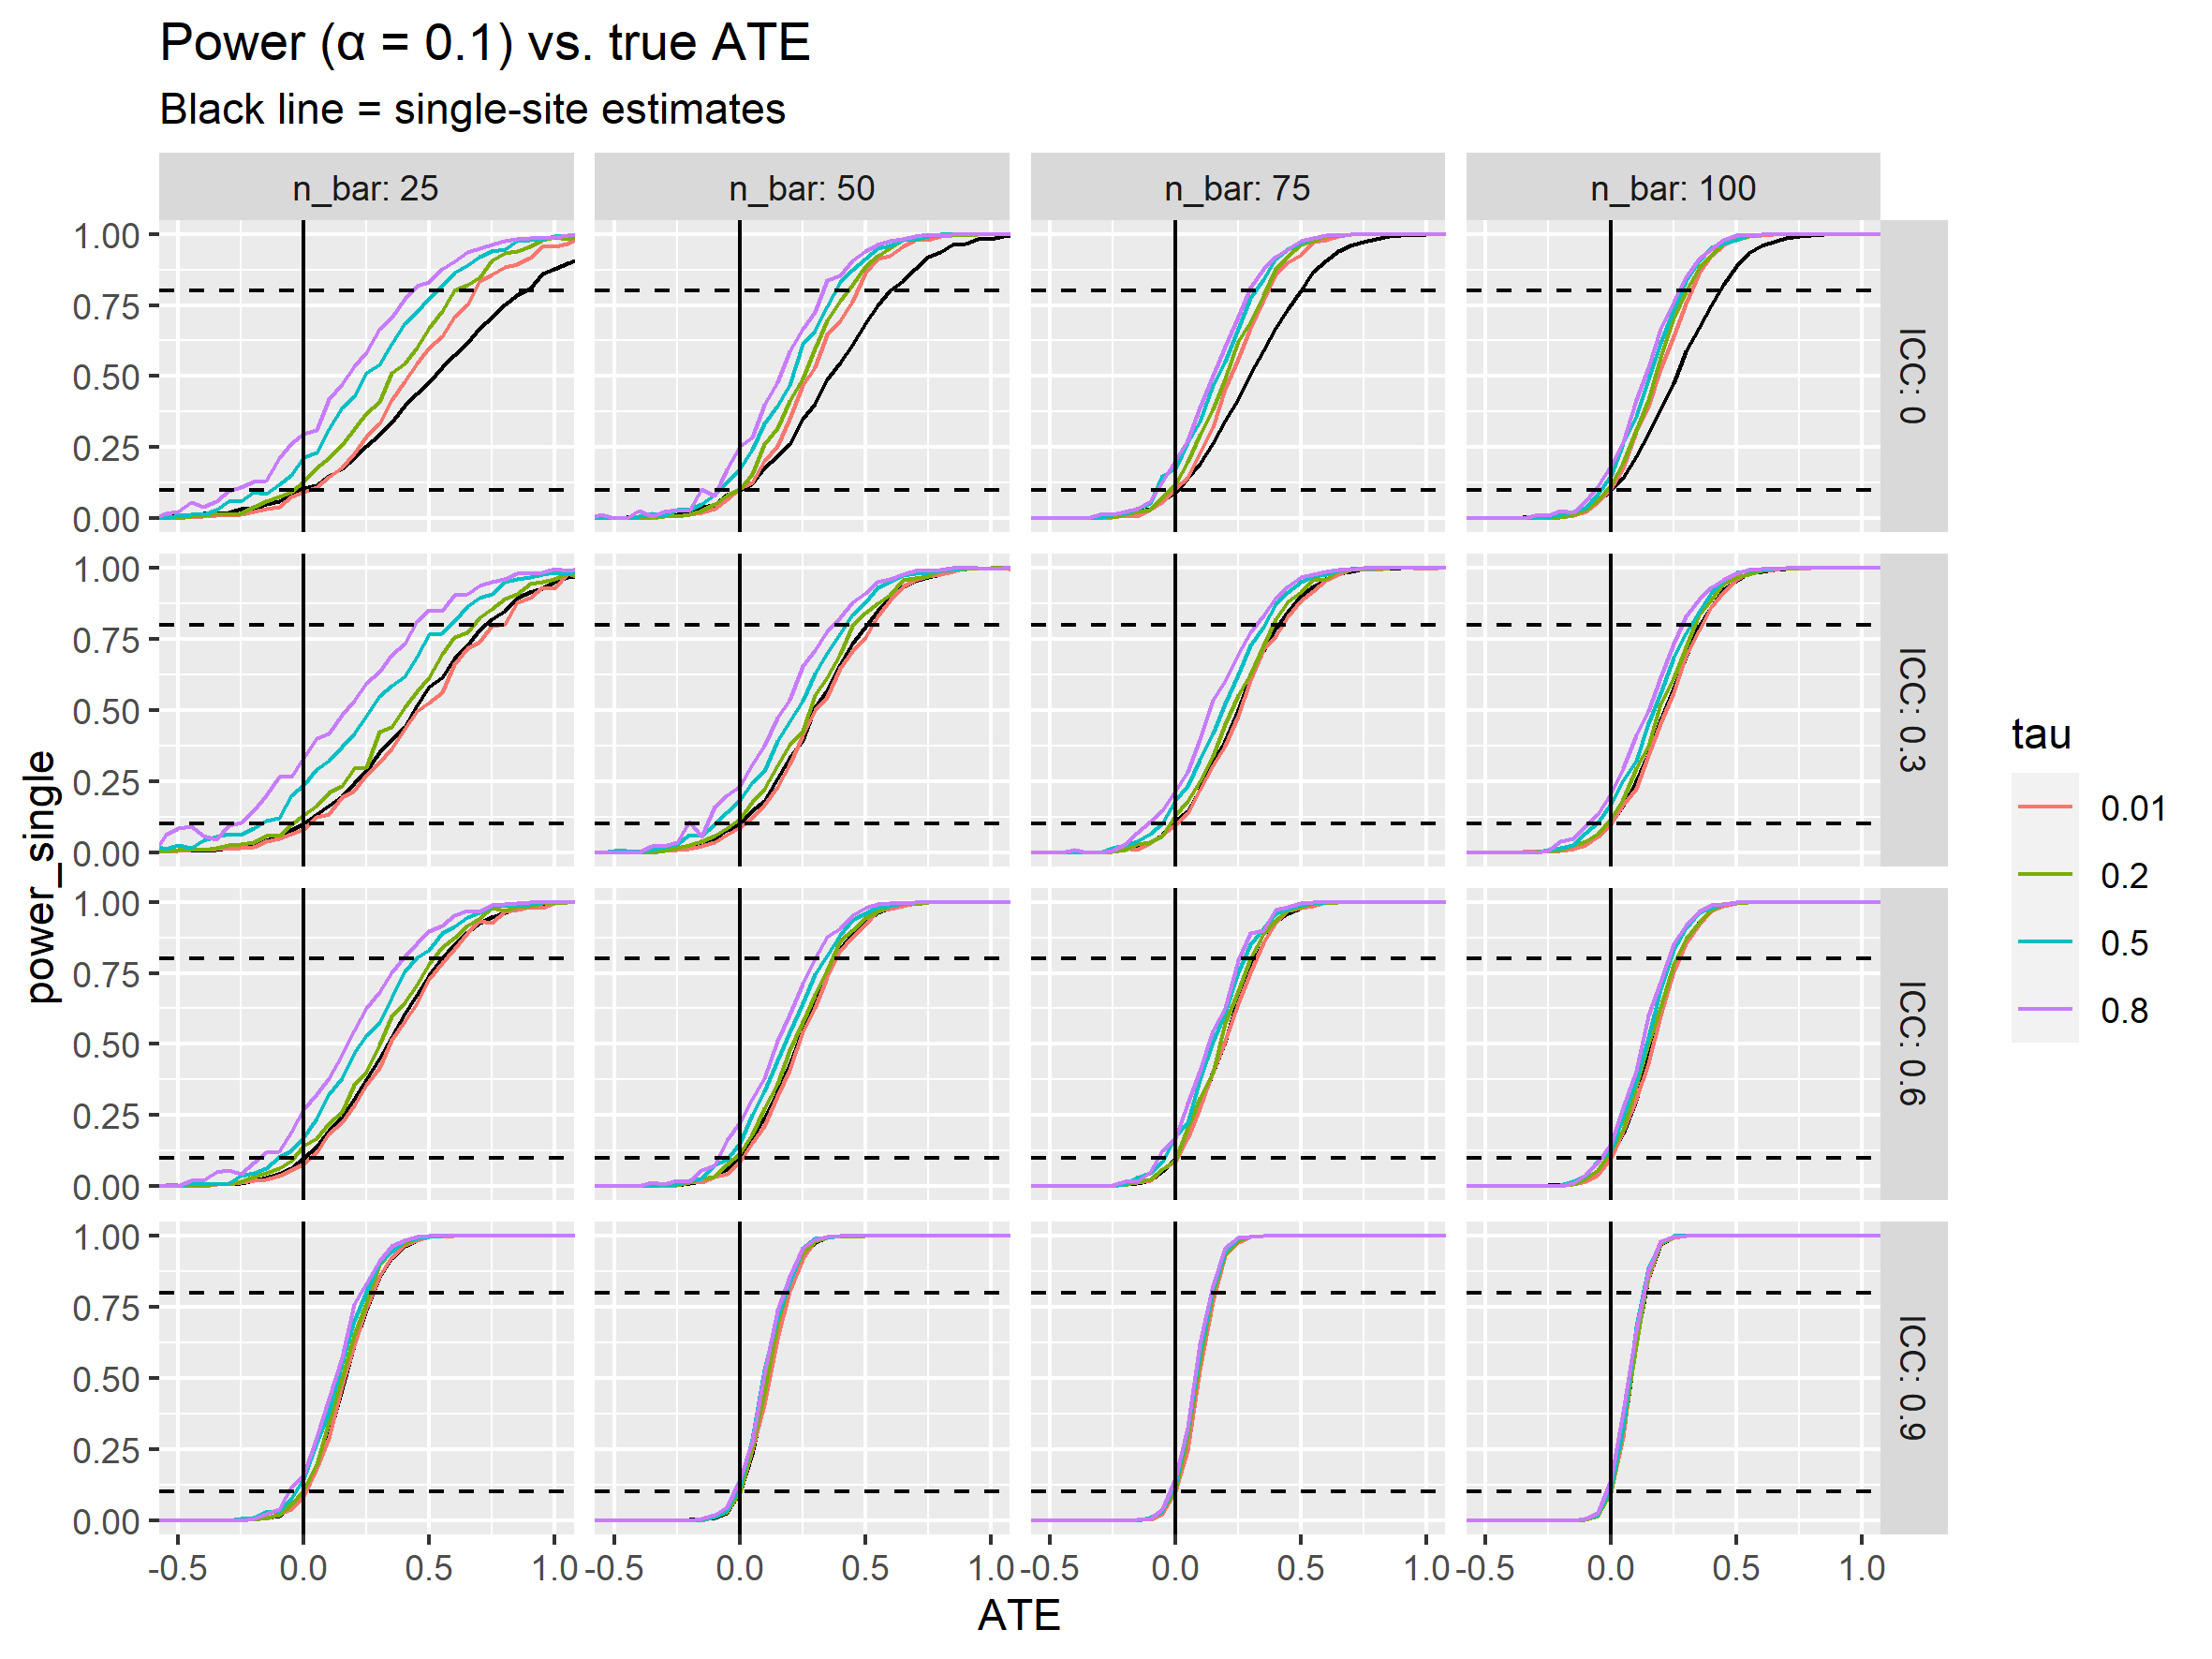
\includegraphics[width=\textwidth]{power_plot_comp}
	\caption{Plot of power (at $\alpha = 0.1$) vs. true site ATE}
	\label{fig:power_plot}
\end{figure}


\begin{figure}[ht]
	\centering
	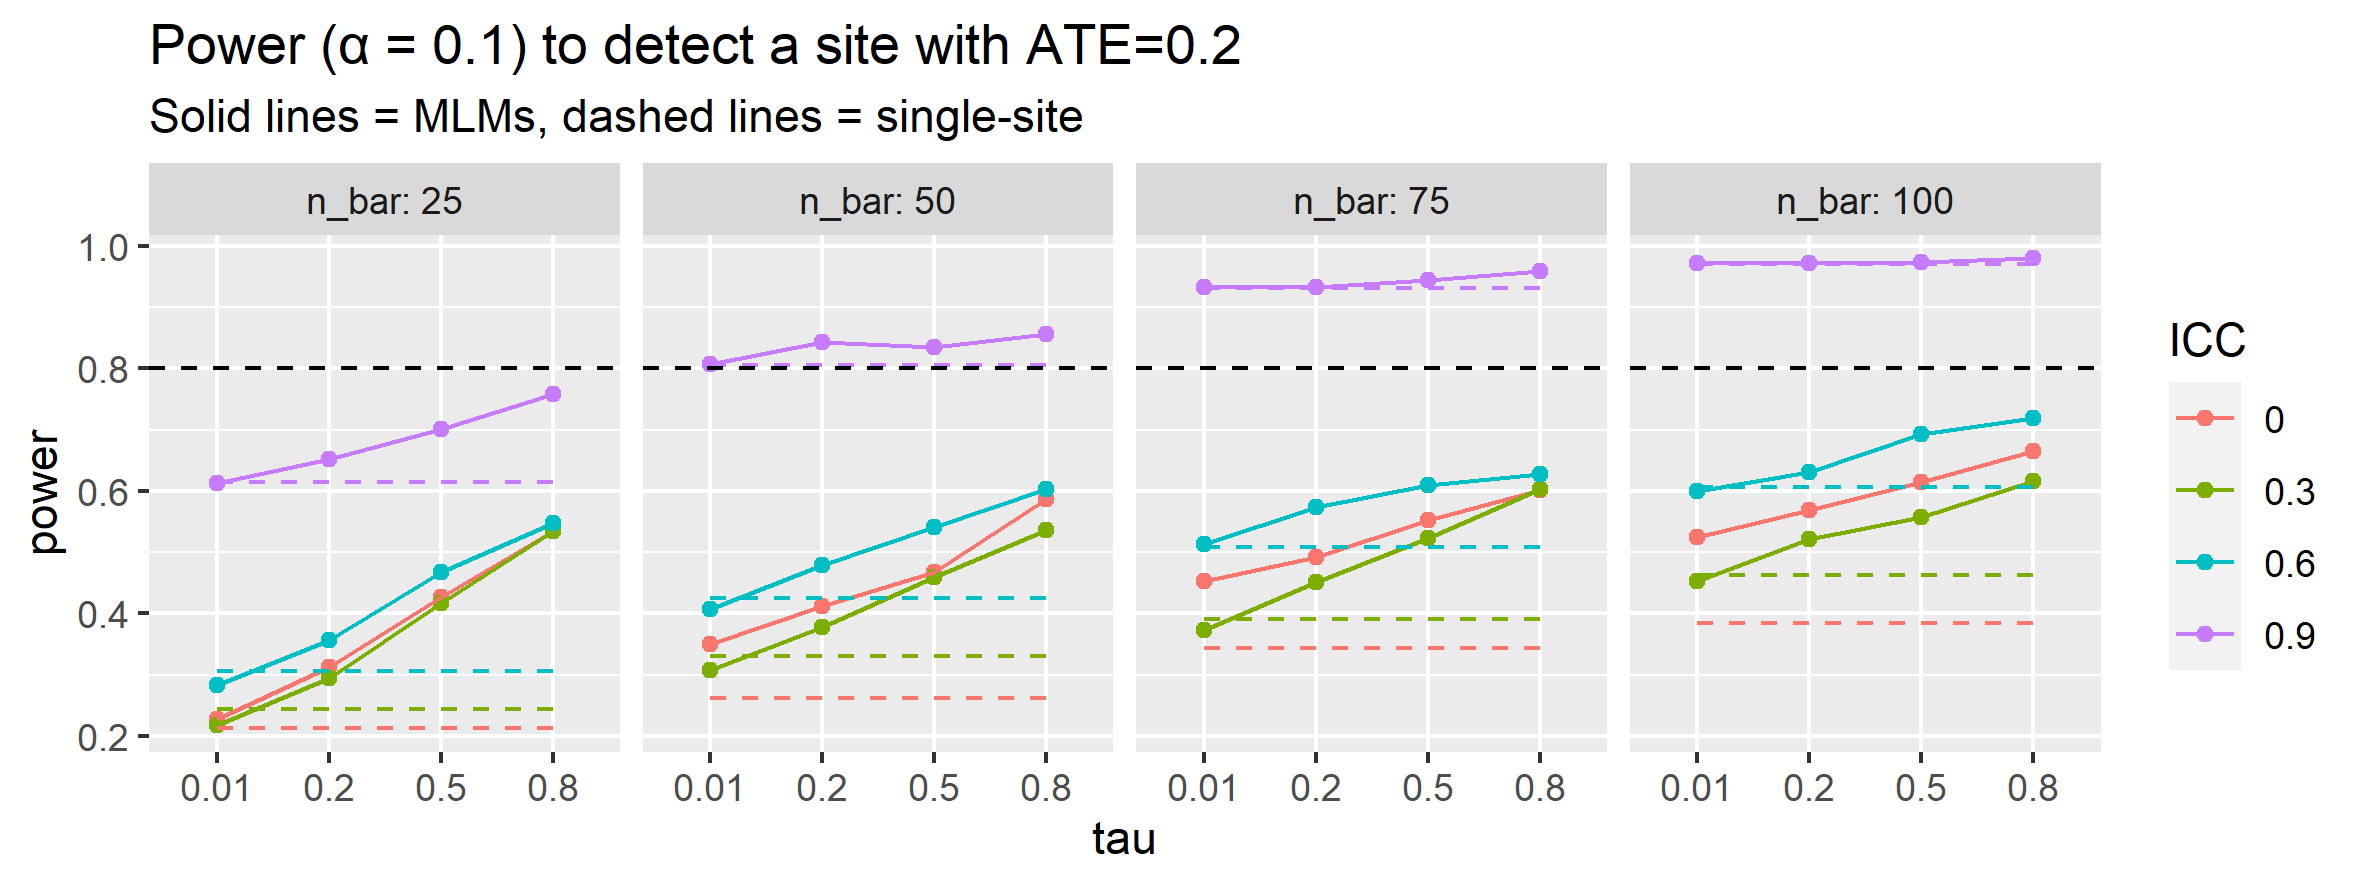
\includegraphics[width=\textwidth]{power_plot_comp_ATE02}
	\caption{Plot of power (at $\alpha = 0.1$) vs. overall average ATE ($\tau$) for sites with $\tau_j = 0.20$}
	\label{fig:power_plot_ATE02}
\end{figure}


\subsection{Results}


Primary results are shown in Figure~\ref{fig:power_plot} and Figure~\ref{fig:power_plot_ATE02}.
The first figure shows power curves as a function of the true average treatment effect for an individual site.
The second figure shows power curves for a site with a true $\tau_j = 0.20$, as a function of the true overall average treatment effect $\tau$.
The solid lines are the MLM models, and the dashed the individual site.

The main trends are as expected: as Figure~\ref{fig:power_plot} shows, power increases as the informativeness of the site data increases, i.e., as $\bar{n}$ or $ICC$ increase, the site-specific standard error (shrunk or otherwise) goes down and power goes up.
We next discuss the power of the MLM models, and then compare that power to the simple-difference models.


\subsubsection{MLM power analyses}

Figure \ref{fig:power_plot} shows the power under various simulation settings, plotted against the true ATE for the site.
As mentioned before, we round the simulated true ATE values $\tau_j$ to the nearest 0.05 before generating student data, so the x-axis in Figure \ref{fig:power_plot} uses the rounded $\tau_j$ values.
The horizontal dashed reference lines are at $\alpha = 0.1$ and $0.80$; ideally, the power curve would approximately follow a step function along the dashed lines, with a rejection rate less than 0.1 for true ATE values less than 0, and a rejection rate over 0.8 for true ATE values greater than 0.

We see that as $\bar{n}$ and $ICC$ increase, the power curve approaches the desired step function, as expected.
We also note that MLM shrinkage has a strong effect when information is low (i.e., $\bar{n}$ and/or $ICC$ are low): for high values of $\tau$, the $\tau_j$ estimates are pulled upward, which increases power across all $\tau_j$ values.
This increase in power, however, also results in an elevated type-I error rate for the sites with $\tau_j \leq 0$.


In Figure \ref{fig:power_plot_ATE02}, we focus on only those sites for which $\tau_j = 0.2$, i.e., sites with a moderate effect size that we would hope to be able to detect.
We note that only when there is little within-site variation ($ICC$ is high) and/or large sample size ($\bar{n}$ is high) do we achieve a power of 0.8.
Also, when the overall site average impact ($\tau$) is high, the shrinkage does help as shown by the upward slant of the lines.

To more fully examine shrinkage for the $\tau_j = 0.20$ sites, see Figure \ref{fig:power_plot_ATE02_dens}.
This figure shows the density curves of the estimated $\hat{\tau}_j$ values across our simulation settings.
We can see the shift in the distributions to the right in the low-information (low $ICC$, low $\bar{n}$) settings, but not in the high-information settings.

\begin{figure}[ht]
	\centering
	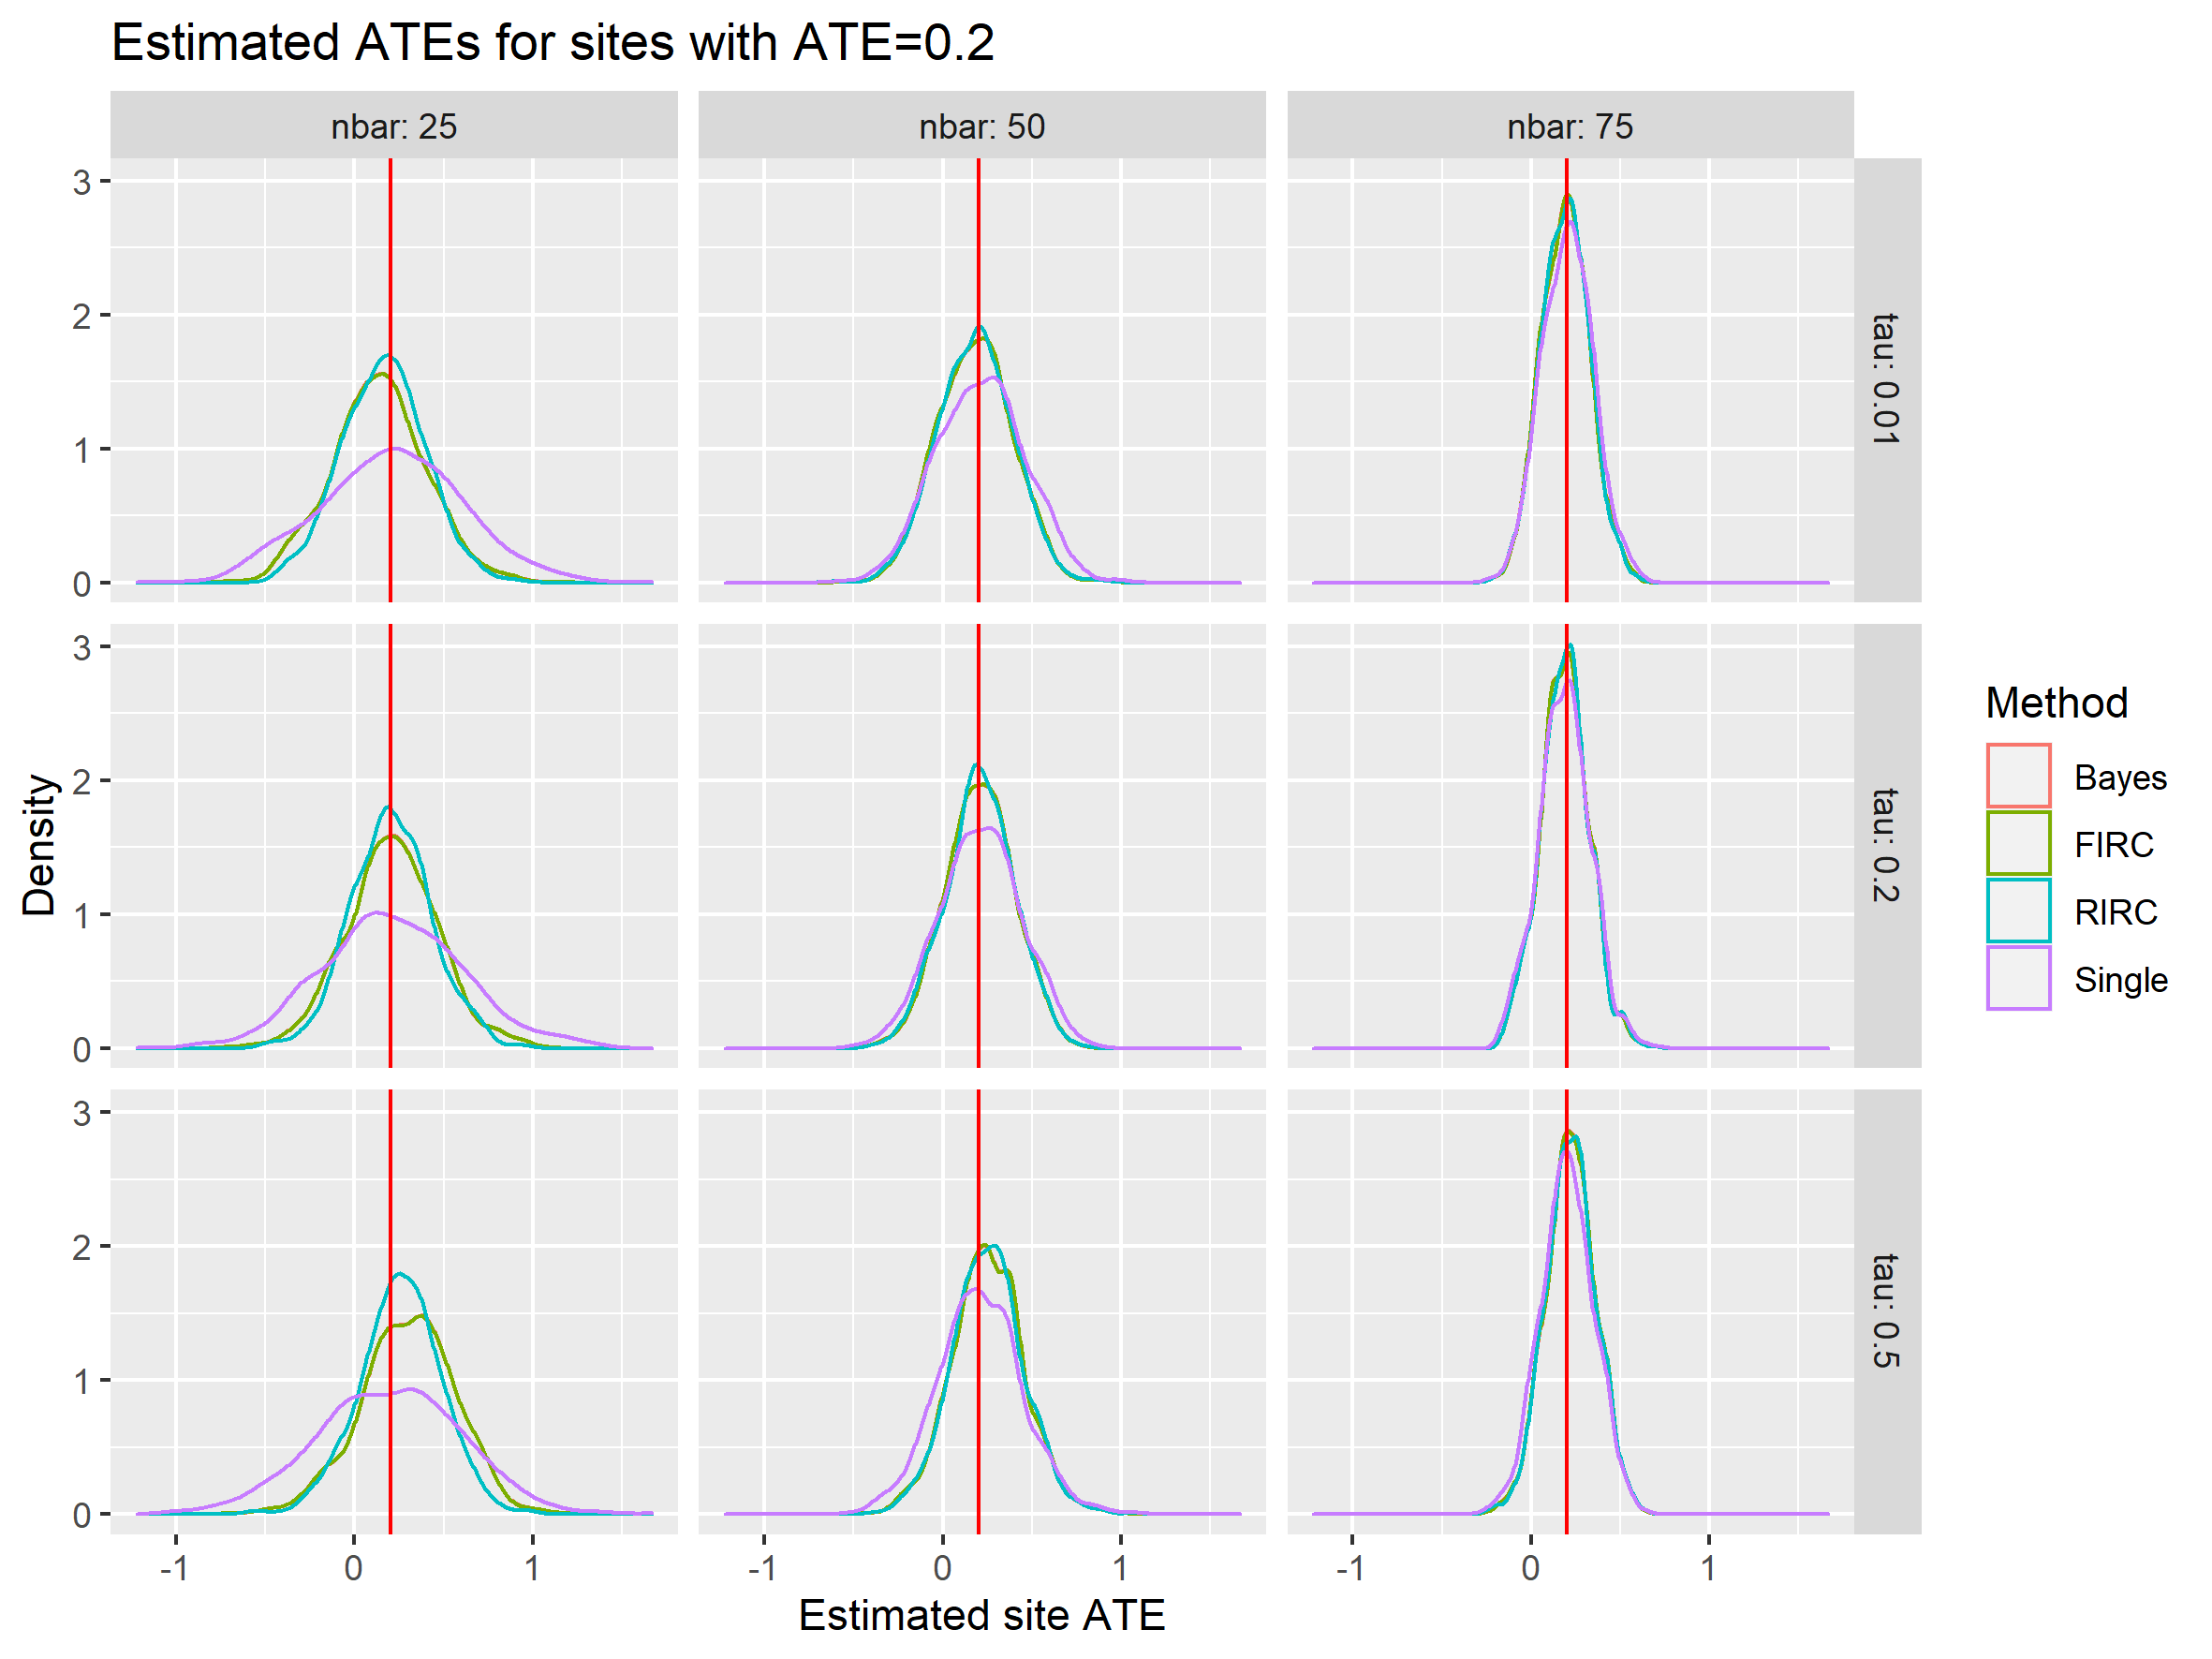
\includegraphics[width=\textwidth]{power_plot_ATE02_dens}
	\caption{Distribution of $\hat{\tau}_j$ for sites with $\tau_j = 0.20$ as a function of overall average impact, ICC, and site size}
	\label{fig:power_plot_ATE02_dens}
\end{figure}


\subsubsection{Comparing MLMs with single-site estimates}

We next compare the power of MLM estimates to the power of single-site estimates, i.e., the treatment-effect estimates we obtain when we ignore the data from the other sites.
We run single-site estimates using a standard Welch's $t$-test with pooled variances.

These single-site estimates are the dashed lines on Figures~\ref{fig:power_plot} and \ref{fig:power_plot_ATE02}.
First we see that MLMs reject either as or more frequently than their single-site counterparts, in all simulation settings tried.
The biggest difference in rejection rates occurs when $\bar{n}$ and/or $ICC$ are low.
In these low-information settings, MLMs have inflated type-I error rates for high values of $\tau$ (i.e., for contexts where the true average impact across sites is large).
When the overall site average is low, however, they have reasonable type-I error rates for when $\tau_j \leq 0$ but still maintain increased power for those sites with larger values of $\tau_j$.


\cmntC{Q: how to interpret? Low $\bar{n}$ means high standard errors. $ICC=0$ means all variation is residual, and not in site intercepts, i.e., higher standard errors.
	This means that we can pool across sites super well, and do better?
	This means that RIRC model has singular intercept fit (probably), and...}

\cmntM{This is an odd result.  Is it due to the high site increasing the average ATE so we are cherry picking samples with overall high sites?  We should do the set site analysis to check, possibly.}

\cmntC{Idea: when $\tau_j$ is higher, it's more likely to come from a simulation where $\bar{\tau}$ is higher, which means upward shrinkage and higher power! This is super annoying. Perhaps doing `set site simulation' will be necessary...}

The dashed horizontal lines on Figure~\ref{fig:power_plot_ATE02} for the $\tau_j = 0.20$ sites show a similar pattern, with the divergence of power increasing as the true average increases, and the divergence increasing more quickly in the low information settings.

Figure~\ref{fig:power_plot_comp_ATE02_dens} compares the single-site estimates and MLM estimates for a $\tau_j=0.20$ site across our $ICC = 0$ scenarios.
This figure shows the impact of shrinkage: the estimated impacts are less spread out and generally closer to the vertical red line denoting 0.20 (the true effect for the site).
As $\tau$ increases, we also see the MLM estimates are shifted toward the right, as expected with shrinkage.
Overall, the MLM model is improving the estimation in terms of how far off the estimate is from the truth.

\cmntM{Perhaps a plot with the RMSE to make this point more forcefully?  In this case, also calculate the RMSE of using the simple estimate average impact for all sites for the site of interest.}



\subsubsection{Discussion}
Overall, MLM shrinkage increases rejection rates, relative to our baseline, when $\tau$ is high and site information is low, which increases both the power and the type-I error rate (type-I error is the rejection rate when the true site impact ($x$-axis) is 0.
For the other settings, however, using a multilevel model does not seem to improve power for one-tailed tests for single sites, when compared to simply running a $t$-test on that site.
In most cases, power is low: MLM is not allowing for any reasonable level of rigor in investigating individual site effects.
That being said, if one really does want a decent guess as to an individual impact, MLM is a far better option, in this context, than the simple difference.


\begin{figure}[ht]
	\centering
	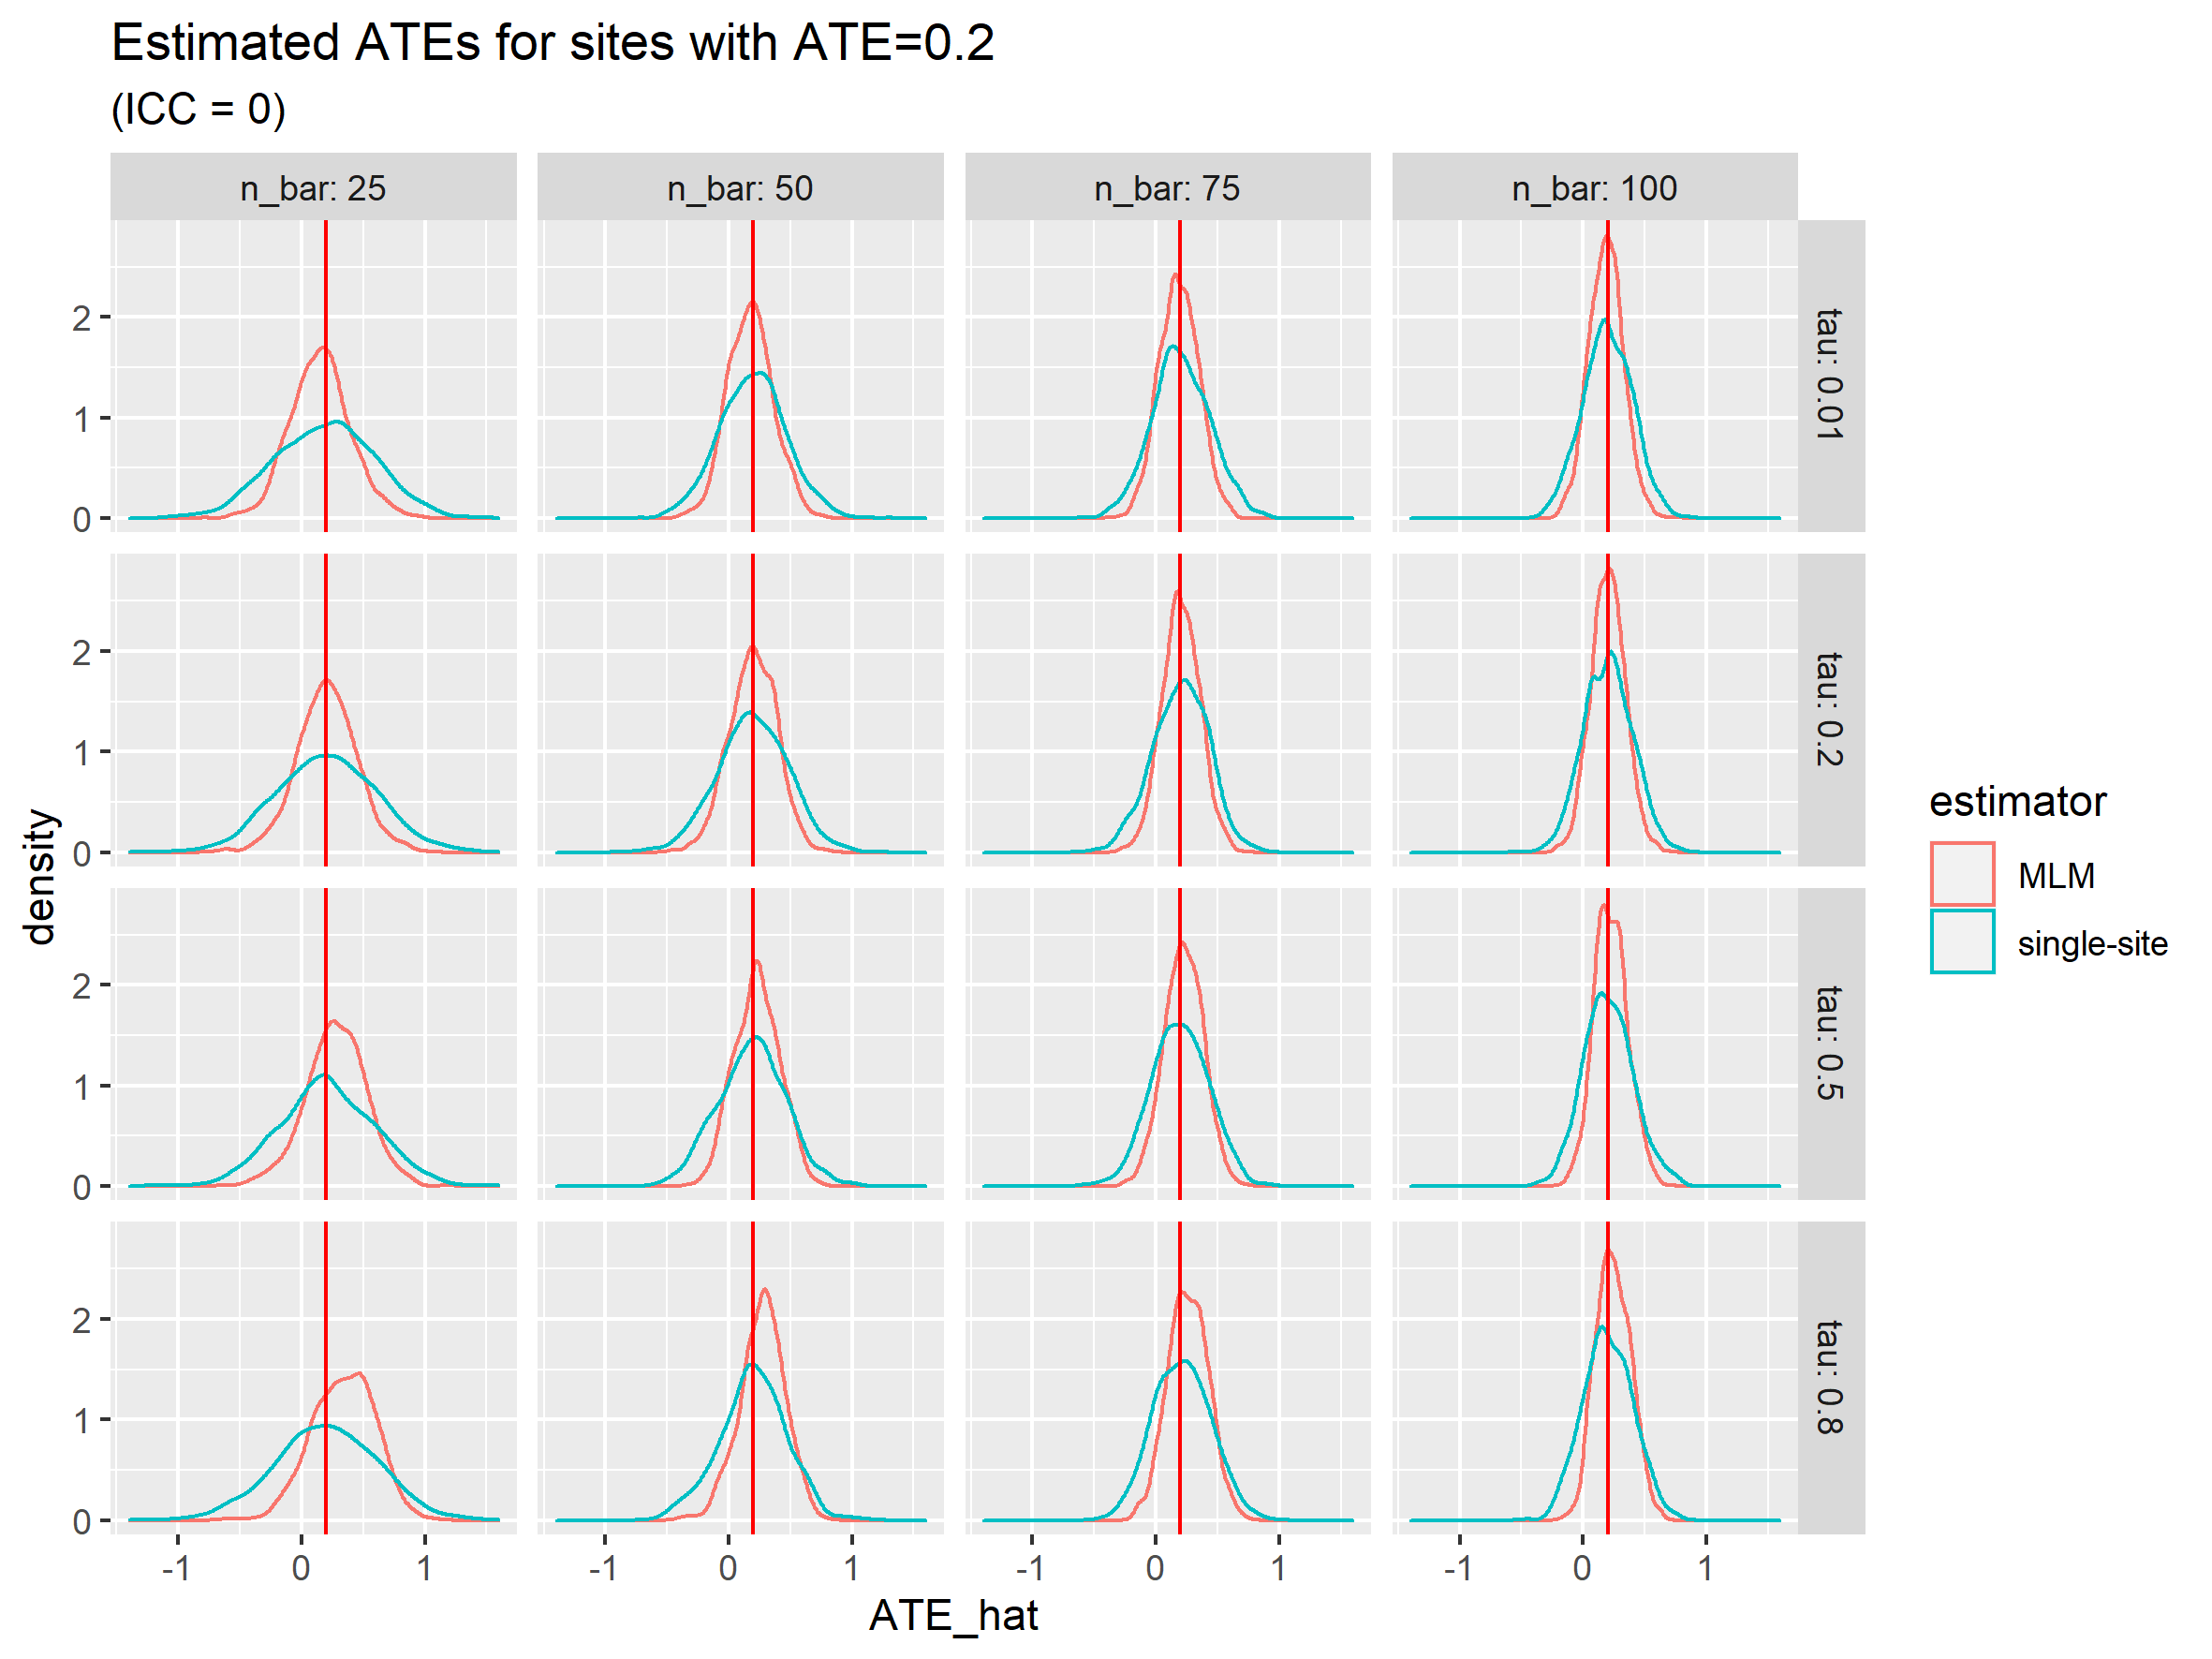
\includegraphics[width=\textwidth]{power_plot_comp_ATE02_dens}
	\caption{Plot of power (at $\alpha = 0.1$) vs. true site ATE}
	\label{fig:power_plot_comp_ATE02_dens}
\end{figure}

\appendix
\section{Appendix A: }

TODOs:
\begin{itemize}
	\item Singular fit rate analysis
	\item Show that rounding $\tau_j$ isn't a horrible sin
\end{itemize}


\cmntM{ Further note: We should perhaps re-do all this with $\tau_j = 0.40$ for a ``big'' effect size, rather than what we might hope is a median site.   This big site would be about 1SD above average in a context with a modest effect and moderate cross site variation.}



	
\end{document}